Navrhněte dvoustupňový operační zesilovač se vstupními tranzistory typu NMOS podle obr. 1, který bude navržen pro tyto vstupní parametry s CL = 10 pF. 

\begin{table}[h]
    \centering
    \caption{Požadované parametry}
    \begin{tabular}{|c|c|c|c|}
        \hline
        \textbf{parametr} & \textbf{hodnota} & \textbf{Vypočítané} & \textbf{Simulace} \\
        \hline
        zesílení ($A_{u0}$) & $\geq 60\ \mathrm{dB}$ & & \\
        \hline
        šířka pásma ($GBW$) & $\geq 10\ \mathrm{MHz}$ & & \\
        \hline
        fázová rezerva ($PM$) & $\geq 60^\circ$ & $60^\circ$ & \\
        \hline
        amplitudová rezerva ($AM$) & -- dB & Nepočítá se & \\
        \hline
        rychlost přeběhu ($SR$)* & $\geq 10\ \mathrm{V}/\mu\mathrm{s}$ & & \\
        \hline
        systematický ofset ($U_{\mathrm{OFF}}$) & $\leq 500\ \mu\mathrm{V}$ & $0$ & \\
        \hline
        spotřeba ($P_{\mathrm{diss}}$) & -- mW & & \\
        \hline
        vstupní napěťový rozsah ($ICMR$) & -- V & & \\
        \hline
        výstupní napěťový rozsah ($OVS$) & -- V & & \\
        \hline
    \end{tabular}
    \\\vspace{1mm}
    \small * pro nástupnou i sestupnou hranu
\end{table}

Vypočítejte a následně simulací zjistěte dosažené parametry z tab. 1. Zobrazte SPICE Output log s parametry všech tranzistorů a vložte jej do protokolu.
Zkontrolujte především gm vstupních tranzistorů a gm7, zda odpovídá výpočtu. 
Dále vložte do protokolu simulační schémata a výstupy simulací ukazující odsimulované hodnoty. 
orovnejte výsledky s ručními výpočty - vytvořte tabulku odsimulovaných a vypočítaných parametrů (viz. Tab. 1 - stejná bude v závěru). 

\vspace{10mm}
\begin{figure}[h!]
    \centering
    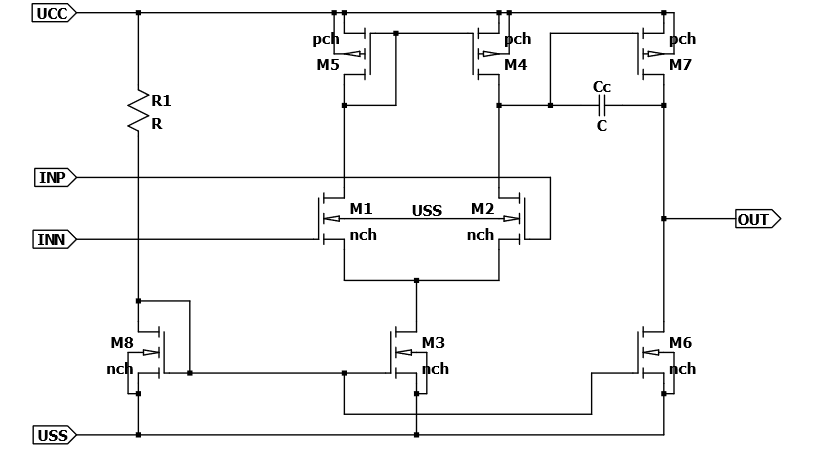
\includegraphics[width=0.6\textwidth]{text/img/zadani.png}
    \caption{\label{fig:res-sch} Schéma zesilovače}
\end{figure}
